\documentclass[oneside]{VUMIFPSkursinis}
\usepackage{algorithmicx}
\usepackage{algorithm}
\usepackage{algpseudocode}
\usepackage{amsfonts}
\usepackage{float}
\usepackage{amsmath}
\usepackage{bm}
\usepackage{caption}
\usepackage{hyperref}
\usepackage{color}
\usepackage{float}
\usepackage{graphicx}
\usepackage{listings}
\usepackage{subfig}
\usepackage{ltablex}
\usepackage{longtable}
\usepackage{wrapfig}
\usepackage{enumitem}
\usepackage{subfig}
\usepackage{caption}
\usepackage{pbox}
\renewcommand{\labelenumii}{\theenumii}
\renewcommand{\theenumii}{\theenumi.\arabic{enumii}.}
\renewcommand{\labelenumiii}{\theenumiii}
\renewcommand{\theenumiii}{\theenumii\arabic{enumiii}.}
% Titulinio aprašas
\university{Vilniaus universitetas}
\faculty{Matematikos ir informatikos fakultetas}
\department{Programų sistemų katedra}
\papertype{Projektinis darbas}
\title{Internetinio banko tinklalapis}
\titleineng{Maketų analitiniai vertinimai}
\status{3 kurso 3 grupės studentai}
\author{Justas Tvarijonas}
\secondauthor{Džiugas Mažulis}   
\thirdauthor{Michal Stankevič}   
\supervisor{Kristina Lapin, Doc., Dr.}
\date{Vilnius – \the\year}

\begin{document}
\maketitle
\sectionnonum{Anotacija}
\subsectionnonum{Darbo tikslas}
Įvertinti 3-ių sukurtų maketų panaudojamumą ir pateikti išvadas, kaip toliau tęsti projektą. Šiam tikslui įgyvendinti išsikėlėme šiuos uždavinius:
\begin{enumerate}
	\item Kiekvienam maketui atlikti euristinį tikrinimą,
	\item Kiekvienam maketui atlikti pažintinę peržvalgą,
	\item Nustatyti tolimesnę projekto eigos kryptį.
\end{enumerate}
\subsectionnonum{Darbo pasiskirstymas}
\begin{itemize}
	\item Justas Tvarijonas - tvarijonasjustas@gmail.com
	\item Džiugas Mažulis - džiugas.mažulis@gmail.com
	\item Michal Stankevič - michal.stankevic@gmail.com 
\end{itemize}
\tableofcontents
\sectionnonum{Įvadas}
\subsectionnonum{Dalykinė sritis}
Internetinė bankininkystė.
\subsectionnonum{Probleminė sritis}
Vartotojo grafinės sąsajos išmokstamumo gerinimas, pagrindinėms funkcijoms pasiekti atliekamų žingsnių bei klaidų mažinimas.
\subsectionnonum{Naudotojai}
Banko klientas - turi galimybę atlikti mokėjimus, peržiūrėti sąskaitos išrašus, kurti mokėjimo ruošinius, ieškoti reikalingos informacijos.
\subsectionnonum{Darbo pagrindas}
Trečiojo laboratorinio darbo reikalavimai.
\section{Džiugo Mažulio maketo vertinimas}
\subsection{Euristinis tikrinimas}
\begin{center}
\begin{longtable}[!htb]{|p{3.5cm}|p{1.9cm}|p{9.6cm}|}
	\caption{Justo Tvarijono vertinimas}
	\endfirsthead
	\endhead
  \hline
	Euristika & Defekto sunkumas & Komentaras \\ \hline
	Būsenos matomumas & 2 & Vartotojas savo buvimo vietą mato tik būdamas pirmame hierarchijos sluoksnyje, jam einant į gylesnius sluoksnius, niekur lange nėra užrašomas esamo lango pavadinimas, nerodomas nukeliautas kelias. \\ \hline
	Sistemos atitikimas realiam pasauliui & 1 & Vietinių mokėjimų lange vartotojui gali būti ne akivaizdu, ką reiškia terminas "Gavėjo pavadinimas" \\ \hline
	Naudotojo valdomas dialogas & 1 & Languose nėra grįžimo atgal mygtukų, vienintelis būdas grįžti yra naudojantis mygtukų juosta. \\ \hline
	Darna ir standartai & 0 & - \\ \hline
	Klaidų prevencija \label{lentele:klaiduPrevencijaJ} & \hyperref[fig:klaiduPrevencijaMygtukai]{4} & 1. Vietinių mokėjimų lange mygtukai "Patvirtinti mokėjimą" ir "Išsaugoti duomenis" nėra atskirti tarpais, bei paspaudus "Patvirtinti mokėjimą" nėra atliekamas papildomas paklausimas ar vartotojas nori atlikti tą mokėjimą, todėl yra galimybė, kad vartotojas norėdamas išsaugoti duomenis prieš savo valią atliks mokėjimo pavedimą. 2. Vietinių mokėjimų lange net neįvedus gavėjo duomenų leidžiama bandyti išsaugoti jo duomenis (tada parodomas klaidos pranešimas, kuriame intuityviai pagal pelės pozicija norisi spausti tą mygtuką, kuris nukelia į pagrindinį langą). Būtų galima išjungti šį mygtuką, kol nėra užpildomi visi privalomi laukai. \\ \hline
	Atpažinimas geriau nei atsiminimas & 0 & - \\ \hline
	Naudojimo lankstumas ir našumas & 1 & Gavėjo sąrašo negalima išrikiuoti pagal poreikius. Galima patobulinimas: leisti vartotojui išrikiuoti gavėjų ruošinius pagal save, kad dažniausiai naudojami/svarbiausi būtų viršuje. \\ \hline
	Estetiškas ir minimalistiniz dizainas & 0 & - \\ \hline
	Remti klaidų atpažinimą, jų priežasčių nustatymą ir taisymą & 1 & Klaidos pranešimuosi vartojamas abstrakčios frazės. \\ \hline
	Pagalba ir dokumentacija & 1 & Mokėjimo lange būtų gerai matyti informaciją apie laukelį į kurį yra vedama reikšmė(ta informacija turėtų aiškiai paaiškinti, kaip turi atrodyti į konkretų laukelį vedami duomenys), tai sumažėtų klaidų/neteisingai įvestų duomenų tikimybė.  \\ \hline
\end{longtable}
\end{center}
\begin{figure}[H]
	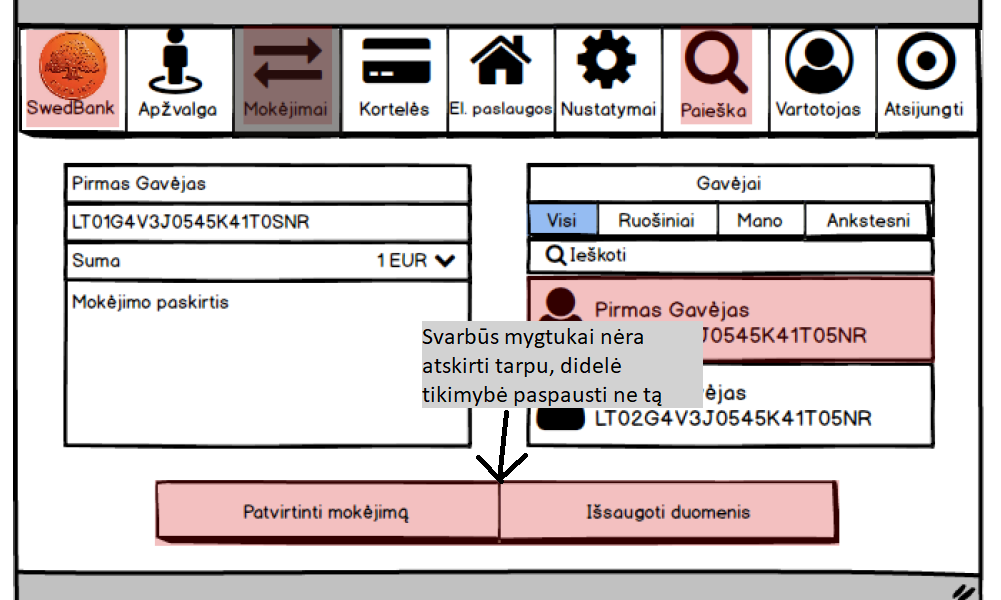
\includegraphics[scale=0.55]{MokejimoPatvirtinimasKlaiduPrevencija.png}
  \caption{Mygtukų išdėstymas vietinių mokėjimų lange}
	\label{fig:klaiduPrevencijaMygtukai}
\end{figure}
\hyperref[lentele:klaiduPrevencijaJ]{Defektas} yra didelės reikšmės, kadangi mokėjimo pavedimas yra rimta operacija, todėl klaidingas jos įvygdymas sukeltų reikšmingų nepatogumų sistemos naudotojui. Šią problemą galima spręsti keliais būdais: 1) mygtukus reiktų atitraukti į priešingas puses, kad tarp jų būtų tarpas užtikrinantis didesnį paspaudimų tikslumą. 2) prieš patvirtinant mokėjimą galima parodyti papildomą langą, kuriame vartotojas galėtų patvirtinti, kad nori atlikti šią operaciją.

\subsection{Pažintinė peržvalga}

\begin{center}
\begin{longtable}[!htb]{|p{5cm}|p{5cm}|p{5cm}|}
	\caption{Justo Tvarijono vertinimas. Mokėjimo pavedimo atlikimas}
\endfirsthead
\endhead
	\hline
	Užduoties žingsniai & Ar aiškiai matoma, ką daryti? & Ar suprantamas atsakas? \\ \hline
	1. Atsidaryti mokėjimų langą & Taip, meniu juostoje mygtukas pavadinimu "Mokėjimai" vartotojui siejasi su jo siekiamu tikslu & Taip, vartotojas gali matyti ar padarė teisingą žingsnį, kadangi šis paspaudimas priartino jį prie tikslo (vartotojas gavo konkretesnius mokėjimo pasirinkimus), bei paspaustas mygtukas pakeitė spalvą. \\ \hline
	2. Pasirinkti vietinius mokėjimus & Taip, tarp lange išdėstytų mygtukų nesunku rasti ieškomą(su pavadinimu "vietiniai mokėjimai") & Nevisiškai, vartotojas, kuris dažniau naudojasi sistema supras, kad yra tame lange, kuriame turi būti, tačiau jame niekur neparašyta, kad tai vietinių mokėjimų langas, tai gali suklaidinti kai kuriuos vartotojus. \\ \hline
	3. Suvesti duomenis & Taip, įvedimo laukai gerai matomi, ant kiekvieno laukelio parašyta, ką jame reikia įvesti(tačiau ant jo paspaudus paaiškinimai digsta) & Ne, sistema niekaip neparodo ar įvesti duomenys yra tinkami. Būtų galima pavaizduoti žalią varnelę prie įvedimo lauko, jeigu duomenys yra validūs. \\ \hline
	4. Patvirtinti mokėjimą & Taip, ekrano apačioje yra mygtukas, kurio tekstas pakankamai aiškiai nurodo, kad jis skirtas mokėjimo patvirtinimui & Taip, patvirtinus mokėjimą išoką patvirtinimo langas, iš kurio vartotojas sužino, kad jo mokėjimas sėkmingai įgyvendintas. \\ \hline
\end{longtable}
\end{center}
\subsection{Apibendrinimas}
% Niekaip neišsiaiškinau ar apibendrinimai turi būt kiekvieno vertintojo atskirai, ar abiejų kartu.
Šio maketo dizainas nenaudoja perteklinių langų, taupiai išnaudoja lango vietą, taip paspartindamas navigaciją. Maketas laikosi darnos, mygtukų išdėstymas bei terminai sutampa visame makete, tačiau yra trūkumų su būsenos matomumu bei klaidų prevencijomis, ko pasekoje išlieka vartotojo pasiklydimo tinklalapyje tikimybė, bei nenorimo veiksmo alikimas. Tačiau pašalinus pagrindinius trūkumus šis maketas(ar tam tikri jo dizaino elementai) gali būti naudojamas.

\section{Justo Tvarijono maketo vertinimas}
\subsection{Euristinis tikrinimas}
\begin{center}
\begin{longtable}[!htb]{|p{3.5cm}|p{1.9cm}|p{9.6cm}|}
	\caption{Džiugo Mažulio vertinimas}
	\endfirsthead
	\endhead
  \hline
	Euristika & Defekto sunkumas & Komentaras \\ \hline
	Būsenos matomumas & 1 & Nėra pagrindinio puslapio indikatorių, todėl šiame lange neaiški vartotojo pozicija. \\ \hline
	Sistemos atitikimas realiam pasauliui & 0 & - \\ \hline
	Naudotojo valdomas dialogas & 0 & - \\ \hline
	Darna ir standartai & 1 & Nerealizuotos ikonos. Maketo 1 puslapyje, pagrindiniame lange, skiltis "Naujienos" užgriozdina langą tekstine informacija. \\ \hline
	Klaidų prevencija & 0 & - \\ \hline
	Atpažinimas geriau nei atsiminimas & 0 & - \\ \hline
	Naudojimo lankstumas ir našumas & 3 & Maketo 7 puslapyje, mokėjimo pavedimo lange, nerealizuotas gavėjų siūlymas pagal kriterijus, vartotojas duomenis turi įvesti pats. Taip pat Maketo 1 puslapyje, pagrindiniame lange, vartotojas nemato sąskaitos bei su ja susijusių duomenų. Kad juos pasiektų vartotojas privalo išskleisti sąskaitos juostą. \\ \hline
	Estetiškas ir minimalistiniz dizainas & 0 & - \\ \hline
	Remti klaidų atpažinimą, jų priežasčių nustatymą ir taisymą & 0 & - \\ \hline
	Pagalba ir dokumentacija & 0 & -  \\ \hline
\end{longtable}
\end{center}

\subsection{Pažintinė peržvalga}

\begin{center}
\begin{longtable}[!htb]{|p{5cm}|p{5cm}|p{5cm}|}
	\caption{Džiugo Mažulio vertinimas. Paieška}
\endfirsthead
\endhead
	\hline
	Užduoties žingsniai & Ar aiškiai matoma, ką daryti? & Ar suprantamas atsakas? \\ \hline
	1. Įvesti paieškos frazę į paieškos teksto lauką & Taip, vartotojui įprastoje vietoje - viduryje viršutinės ekrano dalies - vaizduojama paieškos juosta su padidinimo stiklo ikona. & Taip, įvestas tesktas atvaizduojamas paieškos juostoje.   \\ \hline
	2. Atlikti paiešką & Taip, padidinimo stiklo ikona yra ne tik sutartinis, bet ir intuityvus paieškos funckijos žymėjimas & Taip, sistema užkrauna paieškos rezultatų langą. \\ \hline
	3. Rušiuoti rezultatus & Taip, rezultatų kategorijos vaizduojamos kairėje lango pusėje pabrauktu mėlynos spalvos tekstu & Taip, sistema pavaizduoja pasirinktai kategorijai priklausančius paieškos rezultatus \\ \hline
	4. Atidaryti paieškos rezultatą & Taip, pabraukta mėlynos spalvos rezultato antraštė indikuoja, jog pastarosios paspaudimu vartotojas bus nukreiptas į atitinkamo rezultato langą. & Taip, sistema vaizduoja pasirinką rezultatą su visu jam priklausančiu turiniu. \\ \hline
\end{longtable}
\end{center}

\section{Michal Stankevič maketo vertinimas}
\subsection{Euristinis tikrinimas}
\begin{center}
\begin{longtable}[!htb]{|p{3.5cm}|p{1.9cm}|p{9.6cm}|}
	\caption{Džiugo Mažulio vertinimas}
	\endfirsthead
	\endhead
  \hline
	Euristika & Defekto sunkumas & Komentaras \\ \hline
	Būsenos matomumas & 1 & Maketo 4 puslapyje nenurodyta vartotojo būsena. \\ \hline
	Sistemos atitikimas realiam pasauliui & 0 & - \\ \hline
	Naudotojo valdomas dialogas & 0 & - \\ \hline
	Darna ir standartai & 1 & Egzistuoja iš esmės skirtingos langų temos. \\ \hline
	Klaidų prevencija & 3 & Sujungti tarpusavyje meniu mygtukai kelia gretimos funkcijos pasirinkimo grėsmę. Taip pat maketo 1 lango meniu esantis mygtukas "Paieška" su padidinimo stiklo ikona sufleruoja, jog tai paieškos juosta, o ne mygtukas, atidarantis paieškos puslapį.\\ \hline
	Atpažinimas geriau nei atsiminimas & 1 & Trūksta grafinių elementų, kurie padarytų naršymą efektyvesnį bei intuityvesnį. \\ \hline
	Naudojimo lankstumas ir našumas & 2 & Mokėjimo languose vartotojas neturi galimybės vieno mygtuko paspaudimu pasiekti pagrindiniame meniu vaizduojamas funkcijas. Taip pat atliekant mokėjimo pavedimą vartotojui siūlomi tik ankščiau naudoti gavėjai. Trūksta paieškos rezultatų apdorojamumo. \\ \hline
	Estetiškas ir minimalistinis dizainas & 0 & - \\ \hline
	Remti klaidų atpažinimą, jų priežasčių nustatymą ir taisymą & 0 & - \\ \hline
	Pagalba ir dokumentacija & 0 & Sistema turi sufleruoti vartotojui, jog tam tikruose languose siekdamas grįžti atgal jis turi paspausti ant tuščios vietos. \\ \hline
\end{longtable}
\end{center}

\subsection{Pažintinė peržvalga}

\begin{center}
\begin{longtable}[!htb]{|p{5cm}|p{5cm}|p{5cm}|}
	\caption{Džiugo Mažulio vertinimas. Paieška}
\endfirsthead
\endhead
	\hline
	Užduoties žingsniai & Ar aiškiai matoma, ką daryti? & Ar suprantamas atsakas? \\ \hline
	1. Atsidaryti paieškos langą & Ne, pagrindiniame puslapyje esantį "Ieškoti" mygtuką galima supainioti su paieškos juosta. & Taip, paspaudus mygtuką atidaromas paieškos langas. \\ \hline
	2. Įvesti paieškos frazę į paieškos teksto lauką & Taip, paieškos juostoje parašyta "Įveskite frazę" & Taip, įvesti simboliai atvaizduojami paieškos juostoje. \\ \hline
	3. Atlikti paiešką & Taip, greta paieškos juostos vaizduojamas paryškintas mygtukas "Ieškoti" nepalieka vietos interpretacijoms. & Taip, sistema pavaizduoja paieškos rezultatų langą \\ \hline
	4. Atidaryti paieškos rezultatą & Ne, rezultatų antraštės išsiskiria tik šrifto dydžiu. Vartotojui kyla dvejonių kur derėtų spausti siekiant pasirinkti pageidaujamą paieškos rezultatą. & Ne, paieškos rezultato atidarymas makete neįgyvendintas. \\ \hline
\end{longtable}
\end{center}
\subsection{Euristinis tikrinimas}
\begin{center}
\begin{longtable}[!htb]{|p{3.5cm}|p{1.9cm}|p{9.6cm}|}
	\caption{Justo Tvarijono vertinimas}
	\endfirsthead
	\endhead
  \hline
	Euristika & Defekto sunkumas & Komentaras \\ \hline
	Būsenos matomumas & 0 & - \\ \hline
	Sistemos atitikimas realiam pasauliui & 0 & - \\ \hline
	Naudotojo valdomas dialogas & 0 & - \\ \hline
	Darna ir standartai & 0 & - \\ \hline
	Klaidų prevencija \label{lentele:klaiduPrevencijaM} & \hyperref[fig:klaiduPrevencijaMygtukai2]{4} & 1. Vietinių mokėjimų lange mygtukai "Mokėti" ir "Atidėti" atskirti labai mažu tarpu, bei paspaudus "Mokėti" nėra atliekamas papildomas paklausimas ar vartotojas nori atlikti tą mokėjimą, todėl yra galimybė, kad vartotojas norėdamas atidėti mokėjimą prieš savo valią atliks mokėjimo pavedimą. \\ \hline
	Atpažinimas geriau nei atsiminimas & 0 & - \\ \hline
	Naudojimo lankstumas ir našumas & 0 & - \\ \hline
	Estetiškas ir minimalistiniz dizainas & 1 & Swedbank mygtukas pradiniame lange nėra reikalingas, kadangi jis neatlieka jokio funkcionalumo ir nesuteikia jokios reikalingos informacijos. Grįžimo mygtukas yra pačioje lango apačioje, jį gali uždengti puslapio klostės. \\ \hline
	Remti klaidų atpažinimą, jų priežasčių nustatymą ir taisymą & 0 & - \\ \hline
	Pagalba ir dokumentacija & 1 & Mokėjimo lange būtų gerai matyti informaciją apie laukelį į kurį yra vedama reikšmė(ta informacija turėtų aiškiai paaiškinti, kaip turi atrodyti į konkretų laukelį vedami duomenys). \\ \hline
\end{longtable}
\end{center}
\begin{figure}[H]
	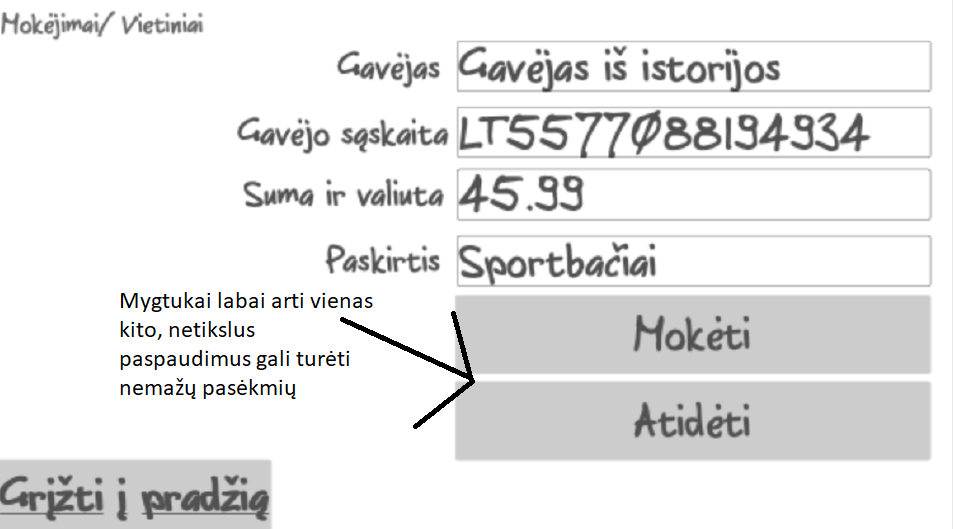
\includegraphics[scale=0.55]{MokejimoPatvirtinimasKlaiduPrevencija2.png}
  \caption{Mygtukų išdėstymas vietinių mokėjimų lange}
	\label{fig:klaiduPrevencijaMygtukai2}
\end{figure}
\hyperref[lentele:klaiduPrevencijaM]{Defektas} yra didelės reikšmės, kadangi mokėjimo pavedimas yra rimta operacija, todėl klaidingas jos įvygdymas sukeltų reikšmingų nepatogumų sistemos naudotojui. Šią problemą būtų galima spręsti prieš mokėjimo įvygdymą pateikiant papildomą patvirtinimo langą.
\subsection{Pažintinė peržvalga}

\begin{center}
\begin{longtable}[!htb]{|p{5cm}|p{5cm}|p{5cm}|}
	\caption{Justo Tvarijono vertinimas. Mokėjimo pavedimo atlikimas}
\endfirsthead
\endhead
	\hline
	Užduoties žingsniai & Ar aiškiai matoma, ką daryti? & Ar suprantamas atsakas? \\ \hline
	1. Atsidaryti mokėjimų langą & Taip, meniu septinkampyje yra mygtukas pavadinimu "Mokėjimai".  & Taip, naujai atsidarame lange vartotojas mato, kad jo pavadinimas yra "Mokėjimai"  \\ \hline
	2. Pasirinkti vietinius mokėjimus & Taip, tarp lange išdėstytų mygtukų nesunku rasti ieškomą(su pavadinimu "Vietiniai") & Taip, pagal duonos trupinių šablono teikiamą informaciją vartotojas, gali matyti, kad atsidūrė vietinių mokėjimų lange. \\ \hline
	3. Suvesti duomenis & Taip, įvedimo laukai gerai matomi, šalia kiekvieno įvedimo lauko parašyta, kokia informacija jame turi būti įvesta & Taip, įvedus visus duomenis atsiranda papildomi mygtukai, kurie leidžia toliau testi užduotį \\ \hline
	4. Patvirtinti mokėjimą & Taip, suvedus duomenis ekrano apačioje atsiradęs mygtukas "Mokėti" sufleruoja apie mokėjimo patvirtinimą & Taip, patvirtinus atsidaro naujas langas, kuriame pranešama apie sėkmingą mokėjimą \\ \hline
\end{longtable}
\end{center}
\subsection{Apibendrinimas}
% Niekaip neišsiaiškinau ar apibendrinimai turi būt kiekvieno vertintojo atskirai, ar abiejų kartu.
Šis maketas yra minimalistinis, ko pasekoje neturi didelio kiekio defektų euristiniame patikrinime. Maketas inovatyvus pakankamai paprastas naudoti, tačiau jame trūksta pagalbos ir dokumentacijos naujiems vartotojams, o patyruniems vartotojams jis gali pasirodyti per daug paprastas.
\section{Išvados}
\section{Priedai}
	\begin{itemize}
		\item Justas Tvarijonas - VU MIF programų sistemų sistemos 3 kurso studentas.
		\item Džiugas Mažulis - VU MIF programų sistemų sistemos 3 kurso studentas.
		\item Michal Stankevič - VU MIF programų sistemų sistemos 3 kurso studentas.
	\end{itemize}
\end{document}
